\documentclass[tikz,border=8pt]{standalone}
\usepackage{amsmath}
\usepackage{pgfplots}
\pgfplotsset{compat=1.18}
\usetikzlibrary{arrows.meta}
\definecolor{ink}{HTML}{21352F}
\definecolor{teal}{HTML}{087F7B}
\definecolor{gold}{HTML}{C58B2A}
\definecolor{blue}{HTML}{4B77A8}
\definecolor{rose}{HTML}{B65A62}
\begin{document}
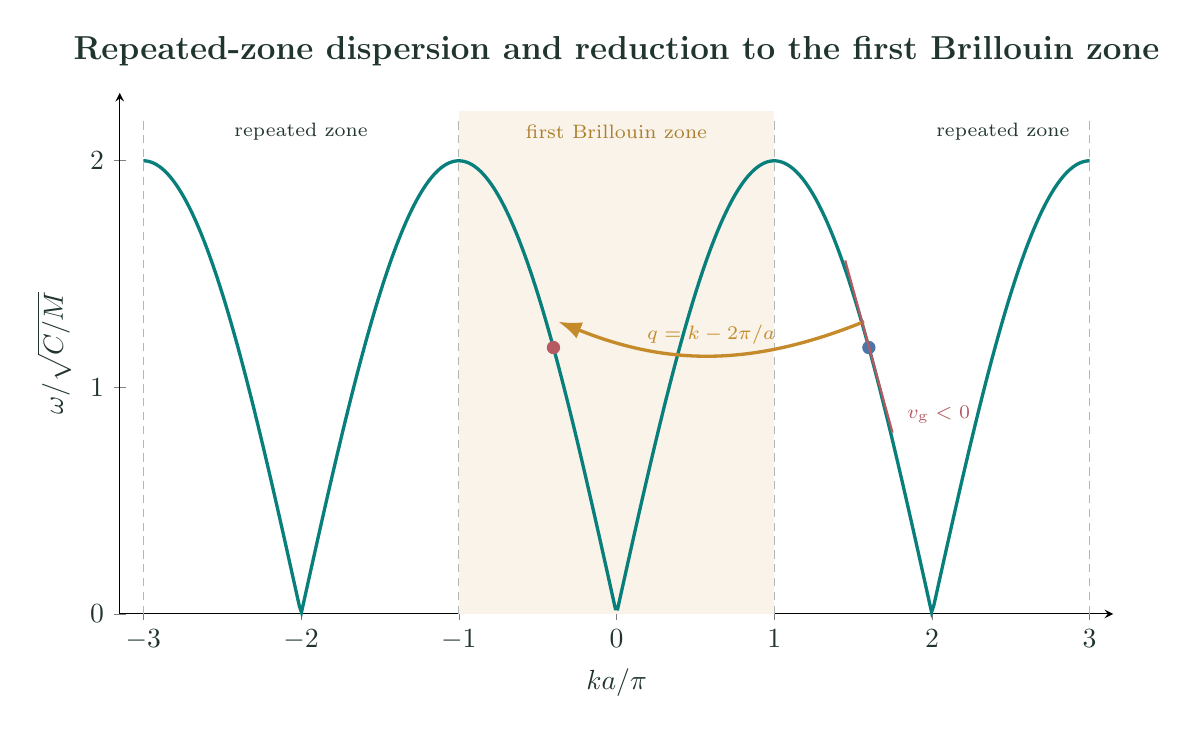
\begin{tikzpicture}[font=\sffamily,text=ink,>=Latex]
\begin{axis}[
  width=14.2cm,height=8.2cm,xmin=-3.15,xmax=3.15,ymin=0,ymax=2.3,
  axis lines=left,xlabel={$ka/\pi$},ylabel={$\omega/\sqrt{C/M}$},
  xtick={-3,-2,-1,0,1,2,3},ytick={0,1,2},
  title={Repeated-zone dispersion and reduction to the first Brillouin zone},
  title style={font=\bfseries\large},clip=false]
  \path[fill=gold!10] (axis cs:-1,0) rectangle (axis cs:1,2.22);
  \draw[ink!35,densely dashed] (axis cs:-3,0)--(axis cs:-3,2.18);
  \draw[ink!35,densely dashed] (axis cs:-1,0)--(axis cs:-1,2.18);
  \draw[ink!35,densely dashed] (axis cs:1,0)--(axis cs:1,2.18);
  \draw[ink!35,densely dashed] (axis cs:3,0)--(axis cs:3,2.18);
  \addplot[teal,very thick,domain=-3:3,samples=420]
    {2*abs(sin(90*x))};
  \draw[blue,fill=blue] (axis cs:1.6,1.1756) circle (2.2pt);
  \draw[rose,fill=rose] (axis cs:-.4,1.1756) circle (2.2pt);
  \draw[->,gold,very thick] (axis cs:1.57,1.29) to[bend left=22]
    node[midway,above,font=\scriptsize] {$q=k-2\pi/a$} (axis cs:-.37,1.29);
  \draw[rose,thick] (axis cs:1.45,1.56)--(axis cs:1.75,.80);
  \node[rose,font=\scriptsize,anchor=west] at (axis cs:1.78,.88) {$v_{\rm g}<0$};
  \node[gold!85!ink,font=\scriptsize] at (axis cs:0,2.13) {first Brillouin zone};
  \node[font=\scriptsize] at (axis cs:-2,2.13) {repeated zone};
  \node[font=\scriptsize] at (axis cs:2.45,2.13) {repeated zone};
\end{axis}
\end{tikzpicture}
\end{document}
